\documentclass[master=cws,masteroption=ai,inputenc=utf8]{kulemt}
\setup{title={Automatisch vertalen van logigrammen naar logica},
  author={Jens Claes},
  promotor={Prof. dr. M. Denecker},
  assessor={},
  assistant={Dr. B. Bogaerts \and Ir. L. Janssens}}
% De volgende \setup mag verwijderd worden als geen fiche gewenst is.
\setup{filingcard,
  translatedtitle={Automatic translation of logigrams into logic},
  udc=621.3,
  shortabstract={Hier komt een heel bondig abstract van hooguit 500
    woorden. \LaTeX\ commando's mogen hier gebruikt worden. Blanco lijnen
    (of het commando \texttt{\string\pa r}) zijn wel niet toegelaten!
    \endgraf \lipsum[2]}}
% Verwijder de "%" op de volgende lijn als je de kaft wil afdrukken
%\setup{coverpageonly}
% Verwijder de "%" op de volgende lijn als je enkel de eerste pagina's wil
% afdrukken en de rest bv. via Word aanmaken.
%\setup{frontpagesonly}

% Kies de fonts voor de gewone tekst, bv. Latin Modern
\setup{font=lm}

% Hier kun je dan nog andere pakketten laden of eigen definities voorzien
\usepackage[dutch]{babel}
\usepackage{pgf-pie}
\usepackage{url}
\usepackage[T1]{fontenc}
% \usepackage[utf8]{inputenc}
\usepackage{amsthm}
\usepackage{amsmath}
\usepackage{qtree}
\usepackage{footnote}

\theoremstyle{definition}
\newtheorem{ex}{Voorbeeld}[section]

\newcommand{\example}[1]{\textit{``#1''}}

\newcommand{\fstructure}[1]{\left [\begin{tabular}{lr}#1\end{tabular}\right]}
\newcommand{\feature}[2]{#1 & #2 \\}
\newcommand{\fvariable}[1]{\framebox{#1}}

\newcommand{\drsTable}[4]{\begin{table}[h]
  \centering
  #4
  \caption{#1}
  \label{drs:#2}
  #3
\end{table}}
\newcommand{\drs}[2]{
  \begin{tabular}{|l|}
    \hline
    #1 \\
    \hline
    #2 \\
    \hline
  \end{tabular}
}
\newcommand{\ifdrs}[4]{
  \begin{tabular}{@{}lcl}
    & & \\
    \drs{#1}{#2} $\Rightarrow$ \drs{#3}{#4} \\
    & & \\
    % \hline
    % #1 & & \\
    % \hline
    % #2
    % #3 & $\Rightarrow$ & #4 \\
    % & & \\
    % \hline
  \end{tabular}
}


% Tenslotte wordt hyperref gebruikt voor pdf bestanden.
% Dit mag verwijderd worden voor de af te drukken versie.
\usepackage[pdfusetitle,colorlinks,plainpages=false]{hyperref}

%%%%%%%
% Om wat tekst te genereren wordt hier het lipsum pakket gebruikt.
% Bij een echte masterproef heb je dit natuurlijk nooit nodig!
\IfFileExists{lipsum.sty}%
 {\usepackage{lipsum}\setlipsumdefault{11-13}}%
 {\newcommand{\lipsum}[1][11-13]{\par Hier komt wat tekst: lipsum ##1.\par}}
%%%%%%%

%\includeonly{hfdst-n}
\begin{document}

% \begin{preface}
%   Dit is mijn dankwoord om iedereen te danken die mij bezig gehouden heeft.
%   Hierbij dank ik mijn promotor, mijn begeleider en de voltallige jury.
%   Ook mijn familie heeft mij erg gesteund natuurlijk.
% \end{preface}

\tableofcontents*

\begin{abstract}
  In dit \texttt{abstract} environment wordt een al dan niet uitgebreide
  samenvatting van het werk gegeven. De bedoeling is wel dat dit tot
  1~bladzijde beperkt blijft.

  \lipsum[1]
\end{abstract}

% Een lijst van figuren en tabellen is optioneel
%\listoffigures
%\listoftables
% Bij een beperkt aantal figuren en tabellen gebruik je liever het volgende:
\listoffiguresandtables
% De lijst van symbolen is eveneens optioneel.
% Deze lijst moet wel manueel aangemaakt worden, bv. als volgt:
\chapter{Lijst van afkortingen en symbolen}
\section*{Afkortingen}
\begin{flushleft}
  \renewcommand{\arraystretch}{1.1}
  \begin{tabularx}{\textwidth}{@{}p{12mm}X@{}}
    CNL   & Constructed Natural Language \\
    DCG   & Definite Clause Grammars \\
    DRT   & Discourse Representation Theory \\
    DRS   & Discourse Representation Structures \\
    KBS   & Knowledge Base Systems \\
  \end{tabularx}
\end{flushleft}
\section*{Constituenten}
De verschillende soorten constituenten die kunnen voorkomen in een grammatica (terminologie uit de taalkunde). We gebruiken de Engelse afkortingen voor gelijkaardigheid met de literatuur.
\begin{flushleft}
  \renewcommand{\arraystretch}{1.1}
  \begin{tabularx}{\textwidth}{@{}p{12mm}X@{}}
    s     & Sentence (zin) \\
    np    & Noun Phrase (naamwoordgroep) \\
    vp    & Verb Phrase (verbale constituent) \\
    v     & Verb (werkwoord) \\
    iv    & Intransitive Verb (onovergankelijk werkwoord) \\
    tv    & Transitive Verb (overgankelijk werkwoord) \\
    pn    & Proper Noun (eigennaam) \\
    n     & Noun (zelfstandig naamwoord) \\
    det   & Determinator \\
  \end{tabularx}
\end{flushleft}

\section*{Symbolen}
\begin{flushleft}
  \renewcommand{\arraystretch}{1.1}
  \begin{tabularx}{\textwidth}{@{}p{12mm}X@{}}
    $@$   & Applicatie uit lambda-calcalus \\
  \end{tabularx}
\end{flushleft}


\chapter{Inleiding}
\paragraph{} Logigrammen zijn een soort van puzzels waarbij de lezer een aantal zinnen voorgeschoteld krijgt. De zinnen bevatten een aantal concepten (zoals nationaliteit, dier, kleur, ...) en een aantal voorbeelden van die concepten (Noor, Brit, kat, hond, rood, blauw, ...). Tussen elk paar van concepten is er \'e\'en bijectie. De zinnen vormen beperkingen op die bijecties. Het doel van de puzzle is het achterhalen van de waarde van de bijecties. M.a.w. welke voorbeelden van de concepten bij elkaar horen. Bijvoorbeeld ``De Noor woont in het blauwe huis en heeft een kat als huisdier''.

De zinnen van logigrammen zijn redelijk gestructureerd waardoor het mogelijk is om ze automatisch om te vormen naar een meer formele representatie waar een computer mee overweg kan. Deze thesis onderzoekt hoe haalbaar deze automatische vertaling van logigrammen naar logica is.

\chapter{Motivatie}

\paragraph{} Vele bedrijfsprocessen worden geregeld door specificaties. Deze worden vaak geschreven in een natuurlijke taal, door een domein expert. Vervolgens worden deze specificaties vertaald naar uitvoerbare programma's. Bij deze vertaling kunnen er fouten insluipen. Bovendien zijn er vaak meerdere programma's die elk opnieuw de specificatie moeten implementeren. Zo ontstaan er niet alleen inconsistenties met de specificatie, maar ook tussen de verschillende programma's onderling. Ten slotte is het moeilijk om de specificatie achteraf nog aan te passen omdat alle programma's dan aangepast moeten worden.

\paragraph{} Het antwoord van de academische wereld op deze problemen, is het \textit{Knowledge Base}-paradigma. In dit paradigma staat een kennisbank centraal. Deze kennisbank bevat de kennis over de wereld (i.e. de specificatie). Deze kennisbank kan dan gebruikt worden in een \textit{Knowledge Base System (KBS)}. Deze systemen bieden ook een aantal inferenties aan die toegepast kunnen worden op deze kennisbanken. Op basis van deze output kunnen de bedrijfsprocessen dan geregeld worden. Om de kennis voor te stellen, kan men gebruik maken van een formele taal (zoals eerste-orde-logica). Zo'n talen hebben een eenduidige semantiek. Er is dus maar \'e\'en mogelijke manier waarop een zin ge\"interpreteerd kan worden. Dit in tegenstelling tot natuurlijke talen waar zelfs simpele zinnen al snel meerdere betekenissen kunnen hebben.

In het Knowledge Base-paradigma moet de specificatie in natuurlijke taal (geschreven door een domein expert) dus vertaald worden naar een vorm waar het KBS-systeem mee overweg kan: de formele specificatie. Deze specificatie wordt slechts eenmaal geschreven en vervolgens wordt ze gebruikt voor alle soorten inferenties. Daardoor is het niet meer mogelijk dat de programma's onderling inconsistent zijn. Ze gebruiken namelijk allemaal dezelfde formele specificatie. Bovendien is ook het aanpassen van de specificatie makkelijker. Enkel de specificatie moet aangepast worden, de programma's blijven hetzelfde.

\paragraph{} Het probleem met deze aanpak is dat er nog steeds een vertaling moet gebeuren van natuurlijke taal naar een formele taal. De specificatie in natuurlijke taal wordt vaak opgesteld door een domein expert die niet vertrouwd is met formele talen. De formele specificatie wordt dan weer opgesteld door een KBS expert. Deze persoon kent formele talen maar heeft een beperkte kennis van het domein. Door deze mismatch van expertise, sluipen er fouten in de vertaling. De domein expert kan namelijk de subtiliteiten van de formele taal niet lezen. Vice versa kent de KBS expert de subtiliteiten van het domein niet.

\paragraph{} De vraag rijst dus of we een formele taal kunnen ontwerpen die toegankelijk is voor domein experten, rijk genoeg is voor praktische problemen en toepasbaar is binnen het KBS paradigma.

\paragraph{} Deze thesis onderzoekt of een formele natuurlijke taal het antwoord is op die vraag. Hieronder verstaan we (een subset van) een natuurlijke taal met een formele, eenduidige semantiek. Talen die een subset zijn van een natuurlijke taal worden ook wel gestructureerde natuurlijke talen of CNL's (naar het Engelse \textit{Constructed Natural Language}) genoemd. Deze talen verschillen van hun gasttaal doordat ze een aantal zinsconstructies niet toelaten. Dit kan bijvoorbeeld de leesbaarheid van een taal verhogen. Voor dit onderzoek zijn deze talen interessant omdat ambigue constructies op die manier verboden kunnen worden. Bovendien is de grammatica van een CNL veel simpeler dan die van de volledige natuurlijke taal, waardoor het makkelijker is om er een parser voor te schrijven. De zinnen die toegestaan zijn in de CNL worden vaak beschreven in een set van \textit{constructieregels}.

Naast constructieregels bevat een formele natuurlijke taal vaak ook interpretatieregels. Deze laatste bepalen hoe een zin die ambigu is in de gasttaal, ge\"interpreteerd moet worden in de nieuwe taal. De moeilijkheid ligt erin om deze regels te beperken in aantal en in complexiteit, zodanig dat de geconstrueerde taal zo dicht mogelijk tegen de gasttaal aanleunt.

% \paragraph{} We zullen deze formele natuurlijke taal opstellen binnen het domein van logigrammen. Hierbij zullen de constructieregels en interpretatieregels zodanig moeten opgesteld worden dat ze de betekenis van de logigrammen juist omzetten naar een formele representatie.

Het grote voordeel van een formele natuurlijke taal is dat natuurlijke taal al gebruikt wordt bij het opstellen van de specificatie. Een voorbeeld van een domein waar specificaties een grote rol spelen is vereistenanalyse. Ook hier zien we dat specificaties vaak in natuurlijke taal worden opgesteld. Zo toont figuur \ref{fig:natural-language-use} het gebruik van natuurlijke taal in vereistenanalyse in 1999. Slechts 5 procent van de specificaties werd toen in een formele taal opgesteld. Al de rest werd in een natuurlijke taal geformuleerd. 16 procent werd zelfs al in een gestructureerde natuurlijke taal opgesteld (niet per se in talen met een eenduidige betekenis voor elke zin).

\begin{figure}
  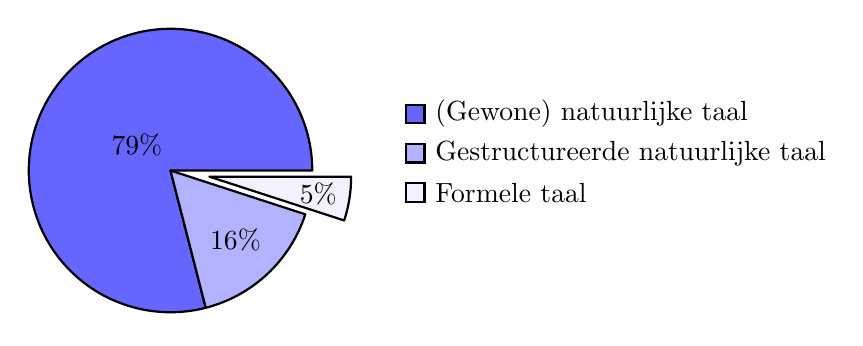
\begin{tikzpicture}
      \pie[text = legend, radius = 1.8, explode = {0, 0, 0.5}, color = {blue!60, blue!30, blue!5}]{79/(Gewone) natuurlijke taal, 16/Gestructureerde natuurlijke taal, 5/Formele taal}
  \end{tikzpicture}
  \caption[Gebruik van natuurlijke taal in vereistenanalyse]{Gebruik van natuurlijke taal in vereistenanalyse in 1999 (van figuur 5 in \cite{Luisa2004})}
  \label{fig:natural-language-use}
\end{figure}

We kozen voor logigrammen als eerste stap in het onderzoek naar zo'n formele natuurlijke taal. Dit omwille van het feit dat logigrammen reeds een beperkte set van zinsconstructies bevat. Bovendien is de evaluatie makkelijker omwille van de veelheid aan logigrammen die men kan vinden.


% Nu begint de eigenlijke tekst
\mainmatter
\chapter{Achtergrond}
Om deze thesis te begrijpen worden hier een aantal concepten uitgelegd die niet per se tot de achtergrondkennis behoren van de lezer. Definite Clause Grammars zijn een soort van grammatica die een aantal voordelen biedt voor het parsen van natuurlijke taal. Feature structures zorgen voor een beperking van het aantal grammaticale regels en verhogen de leesbaarheid ervan. Discourse Representation Theory is een theorie uit de taalkunde voor het vatten van de betekenis van taal. Het introduceert Discourse Representation Structures, een logica die dichter aanleunt bij de natuurlijke taal.

\section{Definite Clause Grammars}
\label{sec:DCG}
Definite Clause Grammars \cite{Pereira1980} zijn een uitbreiding van contextvrije grammatica's die vaak ingebakken zitten in logische talen zoals prolog. Pereira et al.\ \cite{Pereira1980} geven 3 voorbeelden van hoe DCG's kunnen helpen bij het parsen van natuurlijke talen:

\begin{enumerate}
  \item De woordvorm kan afhankelijk gemaakt worden van de context waarin deze verschijnt. Zo kan men eisen dat een werkwoord in de juiste vervoeging voorkomt.
  \item Tijdens het parsen kan men een boom opbouwen die de semantiek van de zin moet vatten. Deze boom hoeft niet isomorf te zijn met de structuur van de grammatica.
  \item Het is mogelijk om prolog code toe te voegen die extra restricties oplegt aan de grammatica.
\end{enumerate}

\subsection{Een eerste grammatica}
\begin{ex}
  Een voorbeeld van een DCG grammatica is:
  \begin{quote}
    \texttt{s ---> np, vp.} \\
    \texttt{np ---> [ik].} \\
    \texttt{np ---> [hem].} \\
    \texttt{vp ---> v, np.} \\
    \texttt{v ---> [zie].}
  \end{quote}
\end{ex} 
\texttt{s} is het startsymbool en staat voor \texttt{sentence}. \texttt{np} staat voor \texttt{noun phrase} (naamwoordgroep of nominale constituent), \texttt{vp} voor \texttt{verb phrase} (verbale constituent) en \texttt{v} voor \texttt{verb}. Deze grammatica zegt dat een zin bestaat uit een noun phrase gevold door een verb phrase. Een verb phrase is dan weer een werkwoord gevolgd door een noun phrase.

De zin \example{ik zie hem} is onderdeel van deze taal. Maar ook de zin \example{ik zie ik} is deel van de taal. Om dit op te lossen kunnen we argumenten meegeven aan de niet-terminaal \texttt{np}.

\subsection{De woordvorm is afhankelijk van de context}
\begin{ex}
  \label{ex:nom-acc-features}
  Deze verbeterde grammatica houdt rekening met welke woordvorm kan voorkomen in welke context.
  \begin{quote}
    \texttt{s ---> np(nom), vp.} \\
    \texttt{np(nom) ---> [ik].} \\
    \texttt{np(acc) ---> [hem].} \\
    \texttt{vp ---> v, np(acc).} \\
    \texttt{v ---> [zie].} \\
  \end{quote}
\end{ex} 

De \texttt{nom} en \texttt{acc} slaan hier op de naamvallen \texttt{nominatief} en \texttt{accusatief}. Ze geven aan in welke functie de naamwoordgroepen gebruikt mogen worden binnen een zin.

\subsection{Een boom als resultaat}
\begin{ex} Verder is het ook mogelijk om een boom op te bouwen tijdens het parsen.
  \begin{quote}
    \texttt{s(Tree) ---> np(NP, nom), vp(Tree, NP).} \\
    \texttt{np(ik, nom) ---> [ik].} \\
    \texttt{np(hem, acc) ---> [hem].} \\
    \texttt{vp(Tree, Subject) ---> v(Tree, Subject, Object), np(Object, acc).} \\
    \texttt{v(zien(Subject, Object), Subject, Object) ---> [zie].}
  \end{quote}
\end{ex} 

Bij het parsen van \example{ik zie hem} krijgen we nu volgende boom:

\Tree[.\textit{zien} \textit{ik} \textit{hem} ]

Merk op dat deze boom de structuur van de grammatica niet hoeft te volgen. Het werkwoord wordt hier tot belangrijkste woord van de zin gebombardeerd.

\subsection{Prolog-code in de grammatica}
\begin{ex} Ten slotte is het mogelijk om prolog restricties te embedden in de grammatica door deze prolog goals tussen accolades te plaatsen.
  \begin{quote}
    \texttt{expression(X) ---> factor(X).} \\
    \texttt{expression(X) ---> term(X).} \\

    \texttt{factor(X) ---> numeral(X).} \\
    \texttt{factor(X) ---> numberal(A), [*], factor(B), \{X is A * B\}.} \\
    \texttt{term(X) ---> factor(A), [+], expression(B), \{X is A + B\}.} \\

    \texttt{numeral(X) ---> [X], \{number(X)\}.} \\
  \end{quote}
\end{ex} 

Bovenstaande grammatica kan simpele wiskunde expressies omvormen tot de wiskundige waarde. Zo wordt \texttt{2 + 4 * 5} omgevormd tot \texttt{22} volgens volgende boom. Hierbij wordt de waarde van onder uit de boom naar boven toe gepropageerd via unificatie.

\Tree[.expression(22)
        [.term(22) [.factor(2) [.number(2) 2 ]]
                   +
                   [.expression(20) [.factor(20) [.number(4) 4 ] * [.factor(5) [.number(5) 5 ]]]]]]

De prologcode in de accolades heeft twee functies. Enerzijds berekent die de waarde van een subexpressie zoals een factor of een term. Anderzijds beperkt de prologcode de grammatica. Een \texttt{numeral} bestaat uit 1 token maar enkel als dat token een getal is volgens prolog. Zo'n beperking in prolog kan ook gebruikt worden om uit de beperkingen van een contextvrije grammatica te treden.

\subsection{Conclusie}
\paragraph{} Definite Clause Grammars zijn expressieve grammatica's die uitermate geschikt zijn voor het modelleren van de grammatica van een natuurlijke taal. In deze thesis zullen alle grammatica's dan ook gegeven worden in de vorm van een DCG.

% \paragraph{}Een laatste opmerking bij deze grammatica is de asymmetrische vorm voor factoren en termen. Een factor is bijvoorbeeld niet gedefinieerd als de vermenigvuldiging van 2 factoren. Dit komt omdat DCG's niet enkel definities zijn van grammatica's maar ook een uitvoeringsstrategie hebben. M.a.w. men krijgt er gratis een parser bij. Deze parser werkt, net als prolog, top-down en van links naar rechts. In het geval van links recursieve regels, zou de parser in een oneindige lus kunnen geraken. Het is echter een bekend resultaat dat men een grammatica altijd kan omvormen zodat deze niet langer links recursief is. Dit is dus geen beperking op welke talen voorgesteld kunnen worden.

% \paragraph{} DCG's zonder prolog code zijn zeer declaratief. Men kan ze namelijk ook puur als definitie van een grammatica beschouwen. Zo kan men een chart parser schrijven die gebruik maakt van een DCG als definitie van de grammatica. Chart parsers zijn interessant voor CNL's omdat ze onthouden welke parti\"ele en volledige constituenten ze al gevonden hebben \cite{Kuhn2008}. Daardoor is er geen nood aan backtracking. Men moet zo niet telkens opnieuw bewijzen wat in een andere tak al bewezen was. Een chart parser onthoudt dat \example{een man} een naamwoordgroep is en kijkt hoe het deze woordgroep kan combineren met andere woorden tot parti\"ele of volledige constituenten. Daardoor is een chart parser veel sneller dan de gratis parser van prolog.

% Bovendien kan men uit de parti\"ele constituenten afleiden welke woordcategorie\"en kunnen volgen op een parti\"ele zin. Zo kan de parti\"ele zin \example{Een rode} gevolgd worden door een adjectief of substantief maar niet door een lidwoord of een werkwoord. Op basis hiervan kan men een suggestietool maken die suggesties geeft i.v.m.\ welke woorden kunnen volgen.

% Ten slotte kan men bij het toevoegen van een woord aan een parti\"ele zin, de resultaten van de vorige parse gebruiken. Dit levert een extra performantiewinst op t.o.v.\ de gratis parser in het geval van incrementele parses. Dit is vooral interessant tijdens het schrijven van een zin, waarbij de vorige parti\"ele zin steeds wordt uitgebreid met \'e\'en woord. Een chart parser hoeft in dat geval namelijk enkel te kijken naar dit nieuwe woord en naar wat er in het geheugen is van de vorige parse, niet meer naar de andere woorden in de zin.

\section{Feature structures}
\label{sec:featureStructures}

\paragraph{} Een feature structure is een term uit de taalkunde. Men kan ze zien als \textit{named arguments} voor een niet-terminaal die gebruikt worden om een explosie aan grammaticale regels te voorkomen. Zo kan een \texttt{np} en \texttt{vp} een feature \texttt{getal} hebben dat aangeeft of de woordgroep in het enkelvoud of meervoud staat. De grammaticale regel voor een zin kan dan aangeven dat het onderwerp en werkwoord moeten overeenkomen in getal. Andere features geven bijvoorbeeld de naamval aan van een naamwoordgroep. Blackburn en Striegnitz \cite{NLPCourse} geven de volgende grammaticale regel als voorbeeld (hierbij staat \texttt{CAT} voor de categorie van een woordgroep):

\[
  \fstructure{
    \feature{CAT}{s}
  }
  \rightarrow
  \fstructure{
    \feature{CAT}{np}
    \feature{NAAMVAL}{nom}
    \feature{GETAL}{\fvariable{1}}
  }
  \fstructure{
    \feature{CAT}{vp}
    \feature{GETAL}{\fvariable{1}}
  }
\]

Deze regel zegt dat een zin bestaat uit een \texttt{np} gevolgd door een \texttt{vp}. De \texttt{np} moet de naamval \texttt{nom} hebben. Bovendien moet het getal van de \texttt{np} en de \texttt{vp} unificeren (de \framebox{1} kan men zien als een variabele).

Grammatica's die gebruik maken van feature structures, gebruiken altijd unificatie voor het samenvoegen van meerdere structuren. Niet alle features moeten namelijk altijd een waarde toegekend krijgen. Zo kan een eigennaam voorkomen als onderwerp en als lijdend voorwerp (en heeft dus geen waarde voor de feature \texttt{naamval}). Terwijl \example{ik} enkel als onderwerp kan voorkomen (en dus wel een waarde heeft voor die feature). Zoals in het voorbeeld hierboven kan men door unificatie ook controleren of meerdere woordgroepen dezelfde waarden hebben voor een feature.

\paragraph{} Zoals Shieber et al.\ \cite{Shieber2003} aanhalen, verschillen prolog termen van feature structures enkel in vorm. Zo speelt de volgorde in prolog wel een rol. Ten slotte moet men steeds alle features vermelden, ook als ze ongebonden zijn. Qua expressiviteit voegen ze echter niets toe aan DCG's. Zo is bovenstaande grammaticale regel op basis van feature structures equivalent met volgende DCG-regel:

\[
    \texttt{s ---> np([naamval:nom, getal:Getal]), vp([getal:Getal]).} \\
\]

\paragraph{} Feature structures (en argumenten in DCG's) zijn handig om de explosie van grammatica regels te voorkomen.
\begin{ex}  Een voorbeeld van een grammatica zonder feature structures uit \cite{NLPCourse}:
  \label{ex:explosion}
  \begin{quote}
    \texttt{s ---> np\_{singular}, vp\_{singular}.} \\
    \texttt{s ---> np\_{plural}, vp\_{plural}.} \\
    \texttt{np ---> np\_{singular}.} \\
    \texttt{np ---> np\_{plural}.} \\
    \texttt{np\_{singular} ---> det, n\_{singular}.} \\
    \texttt{np\_{plural} ---> det, n\_{plural}.} \\
    \texttt{vp\_{singular} ---> intransitive\_verb\_{singular}.} \\
    \texttt{vp\_{singular} ---> transitive\_verb\_{singular}, np.} \\
    \texttt{vp\_{plural} ---> intransitive\_verb\_{plural}.} \\
    \texttt{vp\_{plural} ---> transitive\_verb\_{plural}, np.} \\
    \texttt{n\_singular ---> [man].} \\
    ...
  \end{quote}
\end{ex} 
Hierbij staat de \texttt{n} voor zelfstandig naamwoord (van het Engelse \texttt{noun}) en \texttt{det} voor determinator. Deze grammatica can veel korter gemaakt worden door gebruik te maken van feature structures:

\begin{ex}  Een grammatica met feature structures equivalent aan voorbeeld \ref{ex:explosion} (ook uit \cite{NLPCourse})
  \begin{quote}
    \texttt{s ---> np([num:Num]), vp([num:Num]).} \\
    \texttt{np([num:Num]) ---> det, n(num:Num).} \\
    \texttt{vp([num:Num]) ---> intransitive\_verb([num:Num]).} \\
    \texttt{vp([num:Num]) ---> transitive\_verb([num:Num]), np(\_).} \\
    \texttt{n([num:singular]) ---> [man].} \\
    ...
  \end{quote}
\end{ex} 

\paragraph{Conclusie} Door gebruik te maken van feature structures is de grammatica simpeler en leesbaarder. Bovendien hoeft het concept dat een zin bestaat uit een \texttt{np} gevolgd door een \texttt{vp} maar \'e\'en keer te worden uitgedrukt. De feature structures zorgen voor de congruentie in getal van het onderwerp met het werkwoord.

\section{Discourse Representation Theory}
Voor het vertalen van natuurlijke taal naar logica zouden we graag gebruik maken van Frege's compositionality principe: De betekenis van een zin bestaat uit de combinatie van de betekenissen van de delen ervan. Als we eerste-orde-logica als doeltaal van onze vertaling nemen, komen we echter vrij snel in de problemen. Neem bijvoorbeeld de zin ``If a man lives, he breathes''. De vertaling hiervan in eerste-orde-logica is $\forall x. man(x) \Rightarrow breath(x)$. De vertaling van ``a man lives'' is echter $\exists x. man(x)$, wat geen deel uit maakt van de betekenis van de hele zin. Blackburn en Bos \cite{Blackburn2006} geven nog een aantal andere voorbeelden waarvoor DRS-structuren beter geschikt zijn dan eerste-orde-logica (bijvoorbeeld voor het oplossen van anaforische referenties).

Ze suggereren Discourse Representation Structures als alternatief. Deze structuren bestaan uit een lijst van \textit{discourse referents} (woordgroepen waarnaar andere woordgroepen kunnen verwijzen) en een lijst van condities i.v.m. die referenties \cite{Bos2011}. Blackburn en Bos \cite{Blackburn2006} geven o.a. een vertaling van deze DRS-structuren naar eerste-orde-logica. DRS-structuren hebben dus ook een formele betekenis, zoals we verder zullen aantonen, zijn ze echter beter geschikt als doeltaal. Van hieruit kan dan verder vertaald worden naar eerste-orde-logica volgens de vertaling van Blackburn en Bos. Wij hernemen hier hun vertaling als verdere introductie tot deze structuren:

\[
\Bigg(\drs{x_1, ..., x_n}{
  \gamma_1 \\
  ... \\
  \gamma_n
}\Bigg)^{fo} = \exists x_1...\exists x_n\Big((\gamma_1)^{fo} \land ... \land (\gamma_n)^{fo}\Big)
\]

En de vertaling van alle mogelijke condities:

\[\Big(R(x_1, ..., x_n)\Big)^{fo} = R(x_1, ..., x_n)\]
\[\Big(\tau_1 = \tau_2\Big)^{fo} = \Big(\tau_1 = \tau_2\Big)\]
\[\Big(\lnot B)^{fo} = \lnot\Big(B\Big)^{fo}\]
\[\Big(B_1 \lor B_2)^{fo} = \Big(B_1\Big)^{fo} \lor \Big(B_2\Big)^{fo}\]

\[\Big(\drs{x_1, ..., x_n}{\gamma_1 \\ ... \\ \gamma_2} \Rightarrow B\Big)^{fo} =  \forall x_1...\forall x_n\Bigg(\Big((\gamma_1)^{fo} \land ... \land (\gamma_n)^{fo}\Big) \Rightarrow \Big(B\Big)^{fo} \Bigg)\]

De vertaling van ``If a man lives, he breathes'' naar DRS is \\

\drs{}{\ifdrs{X}{man(X) \\ lives(X)}{}{breathes(X)}}

\paragraph{} Merk op dat de betekenis van het deel ``a man lives'' \drs{X}{man(X) \\ lives(X)} wel deel uitmaakt van de betekenis van de hele zin.

\section{Conclusie} Definite Clause Grammars vormen een expressieve grammatica die natuurlijke taal in al haar facetten makkelijk kan modelleren. Feature Structures komen overeen met argumenten in prolog en kunnen gebruikt worden om grammatica's kort en leesbaar te houden. Discourse Representation Structures vormen een representatie die tussen natuurlijke taal en eerste-orde-logica ligt. Ze zijn even expressief als eerste-orde-logica maar een aantal concepten in de natuurlijke taal zijn beter te modelleren met DRS-structuren.


\chapter{Related work}
In het verleden zijn er al meerdere CNL's gemaakt. Sommige zijn ontwerpen om de leesbaarheid van de specificaties te verhogen en hebben geen formele semantiek. Kuhn \cite{Kuhn2014} heeft een classificatieschema ontwerpen voor CNL's genaamd PENS: \texttt{Precision} (hoe ambigu/formeel is de taal), \texttt{Expressivity} (welke problemen kunnen we uitdrukken), \texttt{Naturalness} (hoe vlot leest de taal), \texttt{Simplicity} (hoe simpel is de taal). In dezelfde paper lijst Kuhn ook een heleboel CNL's op met hun geschiedenis en nut alsook hun classificatie volgens het PENS-schema.

Meer in het algemeen is het omvormen van teksten in natuurlijke taal tot formele modellen al gebeurd in verschillende domeinen: in vereistenanalyse, in het paradigma van business rules, binnen de computationele lingu\"istiek en ten slotte in het domein van de kennisrepresentatie.

Deze sectie geeft een kort overzicht van wat er al gebeurd is in al deze domeinen. Voor een completer overzicht van CNL's, verwijzen we naar Kuhn \cite{Kuhn2014}.

\section{Vereistenanalyse}
\paragraph{Circe} De tool Circe \cite{Ambriola1997} wordt gebruikt in vereistenanalyse. De gebruiker moet een vocabularium, een set van substitutieregels en een specificatie in natuurlijke aanleveren. De tool probeert dan steeds de beste substitutieregel te vinden om zo de tekst geleidelijk aan te transformeren naar een formeel model. Het grote voordeel van de methode is dat er regelsets bestaan voor meerdere soorten modellen: data flow modellen, entity-relationship modellen, ...

Verder is het in Circe mogelijk om in het vocabularium woorden te taggen. De regels kunnen hier dan gebruik van maken om te bepalen of ze van toepassing zijn op bepaalde zinnen. Op die manier introduceert Circe types in het vocabularium.

Een voorbeeld (uit \cite{Ambriola1997}): \example{bron/UIT STUURT data/INFO NAAR doel/IN}. De woorden \example{stuurt} en \example{naar} liggen vast in de regelset. De andere 3 woorden komen uit het vocabularium. Deze moeten een bepaalde tag hebben om te matchen met de regel. Er zijn dus drie types in deze zin: entiteiten die informatie kunnen versturen, entiteiten die informatie kunnen ontvangen en informatie die verzonden kan worden.

Circe is niet echt een CNL. Zinnen die niet matchen met een substitutieregel worden ook niet omgezet in een formeel model. De specificatie kan dus zinnen met en zonder formele betekenis mengen. Er is geen sprake van constructieregels. Alleen (delen van) zinnen die matchen met een substitutieregel krijgen een formele betekenis.

\section{Business rules}
Binnen het paradigma van business rules spelen zowel natuurlijke talen als formele talen een grote rol. SBVR Structured English (SBVR-SE) \cite{Levy2013} en RuleSpeak \cite{Ross2009a} zijn 2 CNL's die proberen om ambigu\"iteit in de natuurlijke taal te verminderen. Deze talen focussen echter vooral op het menselijke aspect \cite{Njonko2014}. Het doel van deze talen is om ambigu\"iteit uit de specificatie te halen en niet zozeer om automatisch natuurlijke taal om te zetten naar een formele voorstelling. RuleCNL \cite{Njonko2014} heeft wel dit doel.

RuleCNL splitst de specificatie op in twee delen: een vocabularium en de regels zelf. Het vocabularium bestaat uit substantieven en werkwoorden alsook hoe deze in verhouding staan tot elkaar. Bijvoorbeeld \example{Auto heeft wiel} geeft aan dat er een relatie kan bestaan tussen een auto en een wiel. Het vocabularium in RuleCNL is dus getypeerd. Voor de regels zelf bestaat er een contextvrije grammatica waaraan de zinnen moeten voldoen.

Om de gebruikers te helpen bij het schrijven van de zinnen in RuleCNL, is er een plug-in voor de Eclipse IDE die automatisch zinnen kan aanvullen en de structuur van bestaande zinnen aangeeft door het kleuren ervan. Bovendien is er een visuele representatie van het domein om de gebruiker te helpen bij het schrijven van het vocabularium.

\section{Computationele lingu\"istiek} Er zijn reeds 2 belangrijke CNL's opgesteld die vertaald kunnen worden naar formele modellen: Attempto Controlled English (ACE) en Processable English (PENG). Beide talen lijken op elkaar en hebben gelijkaardige tools om mee te werken. Ze komen ook allebei uit de computationele lingu\"istiek en zijn ingebakken in taalkundige frameworks die gemaakt zijn om de semantiek van natuurlijke taal in het algemeen te vatten. In de papers over ACE en PENG wordt er niet zoveel gesproken over deze taalkundige aspecten omdat een achtergrond in de (computationele) lingu\"istiek verondersteld wordt.

Hierna volgt eerst een bespreking van ACE. Daarna bespreken we PENG. Hierbij ligt de nadruk op de gelijkenissen en verschillen met ACE. We sluiten af met een beschrijving van hoe deze twee talen ge\"implementeerd zijn met een nadruk op de verduidelijking van een aantal taalkundige aspecten die amper aan bod komen in de papers over ACE en PENG.

\subsection{Attempto Controlled English (ACE)}
\paragraph{} Attempto Controlled English \cite{Fuchs2008} is een gestructureerde natuurlijke taal voor kennisrepresentatie. Het is een subset van Engels die naar een subset van eerste-orde-logica vertaalt. Het is een formele taal: elke zin in ACE heeft slechts \'e\'en betekenis, ook al is de zin ambigu in het Engels. Om te bepalen welke van de betekenissen de \textit{correcte} betekenis is, moet men de interpretatieregels volgen. Omdat dit soms nogal ingewikkeld is, kan men gebruik maken van de parafraseertool van ACE. Deze tool zet de interne representatie terug om naar \'e\'en of meerdere zinnen in ACE. Op die manier kan men niet alleen de betekenis van de zin leren, maar ook de taal zelf. Deze parafrasering leunt echter zeer nauw aan bij de formele taal. Hierdoor is ze niet altijd toegankelijk voor iemand zonder een achtergrond in formele talen.

Bijvoorbeeld de zin \example{Everybody is not present.} heeft 2 betekenissen in het Engels: \example{Everybody is absent} en \example{Somebody is absent}. In ACE is de eerste betekenis de \textit{correcte}. Deze zin wordt geparafraseerd als \example{If there is somebody X1 then it is false that X1 is present.} \footnote{De parafrasering komt van de Attempto Parsing Engine (http://attempto.ifi.uzh.ch/ape/)}. Dit is al een vrij moeilijke parafrasering om te begrijpen terwijl de originele zin nog redelijk simpel is.

\paragraph{}ACE is een general purpose CNL: Het bevat een ingebouwd vocabularium. De gebruiker moet dus zelf geen vocabularium opstellen en kan direct beginnen met het schrijven van de specificatie. Het nadeel aan deze aanpak is dat ACE dus ook geen domeinkennis kan gebruiken voor het analyseren van de zinnen. Sommige constructies moeten daarom met een koppelteken geschreven worden. Zo wordt er in \cite{ACEConstructionRules} het voorbeeld gegeven van \example{A student is interested-in a course} en \example{A student is interested in a classroom}.

Op die manier probeert ACE sommige ambigu\"iteiten op te lossen. Een gelijkaardige truc wordt bijvoorbeeld ook gebruikt om de voorrang van \example{en} en \example{of} op te lossen. Standaard heeft \example{en} voorrang. Maar als de \example{en} voorafgegaan wordt door een komma, dan heeft \example{of} voorrang. \cite{ACEConstructionRules} geeft het voorbeeld \example{A client \{enters a red card or enters a blue card\}, and enters a code.}

In andere gevallen kiest ACE gewoon hoe de zin ge\"interpreteerd moet worden op basis van een set van interpretatieregels. Zo slaat de \example{manually} in \example{A customer who {enters a card manually} types a code.} \cite{ACEConstructionRules} op \example{enters} en niet op \example{types} omdat een bijwoord bij voorkeur achter het werkwoord staat. (De parafrasering is in dit geval wel makkelijk te begrijpen maar vrij lang: \example{There is a customer X1. The customer X1 types a code. The customer X1 enters a card manually.}). Merk ook op dat het onbepaalde lidwoord aanleiding geeft tot een existenti\"ele quantor. In dit geval is de universele quantor echter beter geschikt.

\paragraph{} \'E\'en van de sterke punten van ACE is haar coreferentie-analyse. Dit is het onderzoeken van welke woordgroepen naar hetzelfde concept verwijzen. Neem bijvoorbeeld de zinnen \example{Een man heeft een vrouw. Hij is gelukkig.}. Hierin is \example{Hij} een anaforische referentie (een referentie naar een woordgroep die eerder komt) naar \example{een man}. ACE kan deze coreferenties correct analyseren. ACE doet dit door haar embedding in Discourse Representation Theory, een taalkundig framework. Men kan hier redelijk ver in gaan. Zo worden de zinnen \example{There is a red house and there is a blue house. The red house is large.} correct geanalyseerd. Doordat zinnen in ACE als \'e\'en geheel vertaald worden, kan men dus lange zinnen met veel bijzinnen herschrijven in meerdere kortere zinnen. Dit kan de leesbaarheid van een specificatie vergroten.

\paragraph{} Origineel was ACE bedoeld voor het opstellen van specificaties voor software. Ondertussen kent de taal al meerdere toepassingen, in verschillende domeinen. Er zijn ook meerdere tools die overweg kunnen met ACE als input.

Zo is er de Attempto Parsing Engine APE die ACE zinnen omzet naar Discourse Representation Structures. Dit zijn datatypes uit Discourse Representation Theory die de semantiek van de zin bevatten. APE geeft ook een parafrasering van de invoertekst. Zodat de gebruiker kan controleren of de tool de tekst op de juiste manier leest. Bovendien kan APE waarschuwingen geven bij mogelijke problemen. Bijvoorbeeld het gebruik van een anaforische referentie zonder een antecedent waarnaar deze anafoor kan verwijzen.

\paragraph{} Verder is er de Attempto Reasoner RACE. Deze tool kan controleren of een specificatie consistent is. Indien niet, zal de tool zeggen welke zinnen met elkaar in conflict zijn. Op die manier weet de gebruiker dat er een fout is en waar deze zich ongeveer bevindt. Daarnaast kan de tool vragen in natuurlijke taal beantwoorden. RACE antwoordt niet alleen op de vraag maar geeft ook de zinnen die nodig zijn om te bewijzen dat het gegeven antwoord juist is. Ten slotte kan RACE bewijzen of een bepaalde zin het logische gevolg is van de specificatie. Op die manier kan de gebruiker testen of de specificatie correct is.

APE en RACE zijn de twee belangrijkste tools. Er zijn er echter nog veel meer. Zo is er de ACE View Prot\'eg\'e plug-in. Dit is een plug-in die de vertaling tussen Web Ontology Language (OWL) en ACE doet binnen de Prot\'eg\'e-omgeving (een editor voor het maken van ontologi\"en). Op die manier ziet de gebruiker enkel ACE zinnen en hoeft dus de formele OWL taal niet te kennen om met bestaande modellen om te gaan of om nieuwe modellen te maken. Ten slotte is er AceRules. Hiermee kan de gebruiker de zinnen die ge\"impliceerd worden door de specificatie te weten komen.

Over het algemeen is ACE een zeer uitgebreide taal. Veel Engelse zinnen zijn geldige ACE zinnen, echter niet allemaal. Hierdoor is het moeilijk om de taal te leren. Het is immers niet super duidelijk wat toegestaan is en wat niet. Volgens Fuchs et al.\ \cite{Fuchs2008} heeft een gebruiker 2 dagen nodig om de taal te leren.

\subsection{Processable English (PENG)}
\paragraph{} Andere talen zoals PENG \cite{Schwitter2002} zijn makkelijker om te leren dan ACE. PENG is net als ACE een CNL die vertaalt naar DRS-structuren. In tegenstelling tot ACE bevat PENG geen groot ingebouwd lexicon. De gebruiker moet zelf de woorden aanbrengen die gebruikt worden. De gebruiker kan dit doen tijdens het bewerken en moet dus niet op voorhand aangeven wat het lexicon is. De categorie\"en voor deze domeinspecifieke woorden zijn substantief, adjectief, werkwoord of bijwoord. PENG biedt ook de mogelijkheid om synoniemen of afkortingen te introduceren. Op die manier kan de specificatie vlotter gemaakt worden. Men kan echter geen types meegeven in het lexicon. Men kan dus niet zeggen dat het werkwoord \example{ademen} enkel uitgevoerd kan worden doormensen of dieren en niet door objecten. Naast de domeinspecifieke woorden kent PENG een aantal functionele woorden die ingebakken zitten in de taal, zoals lidwoorden en voegwoorden (\example{de man \underline{die}}). Deze woorden helpen PENG om de zinsconstructies te herkennen.

Net zoals ACE kent PENG het principe van constructieregels en interpretatieregels. De constructieregels bepalen welke zinnen deel zijn van de taal. Bij PENG zijn deze regels eenvoudiger omdat de taal zeer simpel gehouden is. Hierdoor is het makkelijker om zinnen te maken in de taal. Over het algemeen lijken de constructieregels van PENG en ACE veel op elkaar.

De interpretatieregels bepalen hoe de zin vertaald wordt naar logica. Zo is er een interpretatieregel voor hoe anaforische referenties opgelost worden. Deze regel is gelijkaardig in ACE en PENG. Andere regels bepalen welke functiewoorden sterker binden. Zowel ACE als PENG gebruiken hiervoor dezelfde volgorde als in eerste-orde-logica. ACE staat wel uitzonderingen toe door het toevoegen van komma's. PENG houdt de taal simpel en staat dit niet toe.

\paragraph{} PENG is makkelijker om te leren dan ACE omwille van ECOLE \cite{Schwitter2003}. Een tool die suggesties geeft over de woordcategorie\"en die kunnen volgen op een bepaalde zin. Zo geeft Schwitter \cite{Schwitter2003} het voorbeeld van \example{Een} dat gevolgd kan worden door een \texttt{adjectief} of een \texttt{substantief}. Indien de gebruiker de woordcategorie niet kent, kan hij doorklikken op die categorie voor een aantal concrete mogelijkheden. Op die manier moet de gebruiker enkel de woordcategorie\"en leren en niet de geldige zinsconstructies.

Naast de suggestietool bestaat er voor PENG, net zoals voor ACE, ook een parafraseertool. Deze tool herschrijft de invoer zodat het duidelijker is hoe PENG de zin begrepen heeft. Anaforische referenties worden bijvoorbeeld omgezet in de naamwoordgroep waarnaar ze verwijzen.

Net zoals voor ACE zinnen is het ook voor een PENG zinnen mogelijk om te controleren of ze een consistente specificatie vormen \cite{Schwitter2004b}. Daarnaast is het mogelijk om te controleren op redundantie. Indien een zin al door een andere zin ge\"impliceerd wordt, hoeft deze niet expliciet deel uit te maken van de specificatie. Op die manier kan de specificatie kort gehouden worden, wat de leesbaarheid verhoogd.

Naast de general purpose CNL bevat PENG ook een subset specifiek voor het semantische web: PENG-D \cite{Schwitter2004}. Deze subset kan vertaald worden naar description logic (OWL DL), een subset van eerste-orde-logica. PENG-D kan dus gezien worden als het alternatief voor de ACE View Prot\'eg\'e plug-in.
Schwitter \cite{Schwitter2006} vermeldt drie klassieke manieren van voorstellen van een ontologie (N-Triples, RDF/XML en OWL Abstract) en toont dan verder aan dat PENG een vierde manier is om hetzelfde voor te stellen. De paper toont dit aan door verschillende constructies uit OWL te mappen op zinnen in PENG. Het grote voordeel van PENG t.o.v. de andere voorstellingswijzen is dat PENG ook leesbaar en begrijpbaar is voor de mens.

\subsection{Implementatie}
\paragraph{} Zowel ACE als PENG zijn ge\"implementeerd in prolog met behulp van Definite Clause Grammars (DCG) en feature structures voor het omzetten van de natuurlijke taal naar DRS-structuren \cite{Fuchs2008, Schwitter2006}.

\paragraph{Definite Clause Grammars} Aangezien zowel ACE als PENG gebruiken maken van prolog voor hun (eerste) implementatie, is de keuze voor DCG's voor de hand liggend omwille van de parser die men er gratis bijkrijgt. In de tools voor ACE en PENG wordt er echter gebruik gemaakt van een chart parser. Deze parser kan tijdens het schrijven van de zinnen, heel snel voorspellen welke woordcategorie\"en kunnen volgen. Dit helpt de gebruiker bij het schrijven van grammaticaal correcte zinnen zonder de taal te moeten kennen. PENG gebruikt zo'n chart parsers in ECOLE \cite{Schwitter2003}. ACE heeft in navolging van PENG ook AceWiki \cite{Kuhn2008} gemaakt, een subset van ACE voor semantische wiki's. Ook AceWiki bevat een suggestietool. Kuhn et al.\ \cite{Kuhn2008} leggen in detail uit hoe zo'n chart parser gemaakt kan worden voor een CNL en vergelijken de performantie van deze parsers met de gratis parser van prolog.

\paragraph{Feature structures} Naast DCG's wordt er in ACE en PENG ook gebruikt gemaakt van feature structures \cite{Shieber2003, NLPCourse}. Binnen ACE en PENG zorgen de feature structures voor de syntactische correctheid van de zinnen in de gasttaal, het Engels. Via unificatie kan men namelijk testen of een bepaalde woordgroep voldoet aan de voorwaarden van de context. De unificatie van de feature \texttt{getal} van het onderwerp en het werkwoord zorgt voor de congruentie in getal van het onderwerp met het werkwoord. Op die manier zijn zinnen die in ACE en/of PENG geldig zijn, ook geldig in het Engels. Zoals sectie \ref{sec:featureStructures} aanhaalt, wordt op deze manier een explosie van het aantal grammaticale regels vermeden.

\paragraph{DRS} Naast feature structures maken ACE en PENG ook gebruik van Discourse Representation Structures. Ze zijn een onderdeel van Discourse Representation Theory. Dit is een taalkundig framework om de semantiek van natuurlijke taal te vatten. Één van de sterke punten van DRS-structuren is het oplossen van coreferenties. \cite{Fuchs2008drs} bevat meer informatie over hoe DRS-structuren gebruikt worden binnen ACE.

Bos \cite{Bos2011} stelt dat DRS-structuren zowel de rol van semantische inhoud als die van tekstuele context spelen. M.a.w.\ met behulp van deze structuren kan men achterhalen wat de semantiek van een tekst is maar tegelijk bieden ze ook een context aan die helpt bij de coreferentie-analyse. Zo wordt tijdens het parsen de semantiek van een zin opgebouwd en tegelijk de coreferenties opgelost.

Concreet bevat een DRS-structuur een lijst van \textit{discourse referents} (woordgroepen waarnaar andere woordgroepen kunnen verwijzen) en een lijst van bepaling i.v.m. die referenties \cite{Bos2011}. \autoref{drs:example} geeft een voorbeeld van zo'n DRS-structuur voor de zin \example{There is a movie which every man loves deeply}. Er zijn in totaal 3 \textit{discourse referents}: \texttt{movie}, \texttt{man} en \texttt{loves}. Merk op dat naar deze laatste verwezen wordt door het bijwoord \textit{deeply}. Deze DRS kan vertaald worden als $\exists A \cdot \bigg(movie(A) \land \forall B \cdot \Big(man(B) \Rightarrow \exists C \cdot \big( loves(C, B, A) \land deeply(C) \big)\Big)\bigg)$

\begin{savenotes}
  \begin{drsFloat}
    \centering
    \drs{A}{
      movie(A) \\
      \ifdrs{B}{man(B)}
            {C}{loves(C, B, A) \\ deeply(C)}
    }
    \caption{Een DRS-structuur voor de zin \example{There is a movie which every man loves deeply.} \protect\footnotemark}
    \label{drs:example}
    \footnotetext{Deze DRS-structuur werd lichtjes aangepast aan de output van APE (http://attempto.ifi.uzh.ch/ape/)}
  \end{drsFloat}
\end{savenotes}


\paragraph{Conclusie} DCG's zijn een uitbreiding op contextvrije grammatica's uit de wereld van logisch programmeren. Feature structures en Discourse Representation Structures zijn concepten uit de lingu\"istiek. Ze worden gebruikt om de natuurlijke taal en haar semantiek te modelleren. Zo helpen feature structures om een explosie van het aantal grammatica regels te voorkomen. Discourse Representation Structures worden dan weer vooral gebruikt om de coreferentie-analyse te vergemakkelijken. Beiden concepten worden gebruikt in de tools rond ACE en PENG omdat deze talen ontstaan zijn in het vakgebied van computationele lingu\"istiek.

\section{Kennisrepresentatie}
\label{sec:ASP}
In het domein van kennisrepresentatie hebben Baral et al.\ \cite{Baral2008} natuurlijke taal reeds vertaald naar Answer Set Programs (ASP). Ze maken hiervoor gebruik van Combinatorische Categorische Grammatica (CCG) en $\lambda$-calcalus. Een CCG bestaat uit een aantal basiscategorie\"en zoals \texttt{s} (zin) en \texttt{np} (naamwoordgroep) en afgeleide categorie\"en zoals \texttt{s/np} \footnote{een \texttt{S/NP} is een woordgroep die indien gecombineerd met een \texttt{np} langs links een zin vormt} en \texttt{(s/np)$\backslash$np} \footnote{een \texttt{(S/NP)$\backslash$NP} is een woordgroep die indien met een \texttt{np} gecombineerd langs links en langs rechts een zin vormt} \cite{Baral2008}. Zo wordt een onovergankelijk werkwoord voorgesteld als een \texttt{s$\backslash$np}. Verder bevat een CCG een aantal regels die bepalen wat de categorie is van een combintatie van woordgroepen. Zo is er een regel die zegt dat $\alpha\beta$ van categorie \texttt{B} is als $\alpha$ categorie \texttt{A} heeft en $\beta$ categorie \texttt{B$\backslash$A} \cite{Baral2008}. Dankzij deze regel kunnen we afleiden dat als we een onovergankelijk werkwoord (\texttt{s$\backslash$np}) langs links combineren met een naamwoordgroep (\texttt{np}), we dan een zin krijgen. Op deze manier kunnen we een parse tree opstellen waarbij we telkens 2 woordgroepen combineren totdat de zin uiteindelijk categorie \texttt{s} krijgt.

Naast een categorie heeft elk woord ook een betekenis uitgedrukt in een uitbreiding op de $\lambda$-calcalus. In deze uitbreiding kunnen ook ASP-expressies voorkomen. De betekenis van een woordgroep is de combinatie van de betekenis van de woorden. Hierbij gebruiken we de CCG parse tree om de volgorde te bepalen. We verduidelijken met een voorbeeld (grotendeels overgenomen uit Baral et al.\ \cite{Baral2008}). We beschouwen het lexicon zoals weergegeven in tabel \ref{table:CCG} voor de zin \example{Birds fly}. Hierin stelt de \texttt{@} de applicatie voor uit de lambda-calcalus. De combinatie van de woorden \textit{birds} en \textit{fly}, is van de categorie \texttt{s} zoals hierboven reeds uitgelegd. De overeenkomstige lamda-expressies moeten nu op een gelijkaardige manier gecombineerd worden: $\lambda_{birds\ fly}=\lambda_{fly}@\lambda_{birds}$.

\begin{table}
  \centering
  \begin{tabular}{|l|l|l|}
    \hline
    Woord & Categorie & $\lambda$-ASP-expressie \\
    \hline
    \hline
    Birds & np & $\lambda x.bird(x)$ \\
    Fly & s$\backslash$np & $\lambda x.fly(X) \leftarrow x@X$ \\
    \hline
  \end{tabular}
  \caption{Een lexicon voor de woorden birds en fly in een CCG grammatica (uit \cite{Baral2008})}
  \label{table:CCG}
\end{table}

\begin{equation}
  \label{eq:lambda}
  \begin{aligned}
  \lambda_{birds\ fly} &= \lambda_{fly}@\lambda_{birds} \\
          &= (\lambda x.fly(X) \leftarrow x@X)@(\lambda x.bird(x)) \\
          &= fly(X) \leftarrow (\lambda x.bird(x))@X \\
          &= fly(X) \leftarrow bird(X)
  \end{aligned}
\end{equation}

Elk woord heeft een betekenis die men kan zien als een ASP-expressie met gaten erin die opgevuld worden door de combinatie met andere woorden. De manier van combineren van de $\lambda$-expressies hangt af van de categorie\"en van de woorden. Het nadeel aan deze aanpak is dat elk woord (minstens) \'e\'en betekenis moeten hebben in het formaat van een $\lambda$-ASP-expressie. Constantini et al.\ \cite{Costantini2010} lossen dit probleem deels op door gebruik te maken van $\lambda$-ASP-expressie-templates. Sommige woorden hebben nog steeds een eigen $\lambda$-ASP-expressie, voor de andere kan er \'e\'en afgeleid worden uit een $\lambda$-ASP-expressie-template. Zo is $\lambda x. <noun>(x)$ de template voor substantieven. Het gedeelte $<noun>$ moet vervagen worden door een specifieke instantie. Het woord \textit{birds} heeft zo nog steeds dezelfde betekenis.

\paragraph{}Zo'n templates werken echter niet voor alle woorden. Daarom hebben Baral et al.\ \cite{Baral2012} een methode bedacht om van de betekenis van een zin en de betekenis van een aantal woorden, de betekenis van andere woorden af te leiden. Ze doen dit niet langer met $\lambda$-ASP-expressies maar vervangen ASP door eerste-orde-logica: $\lambda$-FOL-expressies. De grammatica en manier van combineren blijft echter hetzelfde. Deze techniek gebruiken Baral et al.\ \cite{Baral2012a} om automatisch een grammatica en semantiek te leren voor logigrammen op basis van andere logigrammen en hun vertaling in een ASP programma. Hiervoor gebruiken ze \'e\'en ASP-ontologie die toepasbaar is voor vele logigrammen. Ze bewerken hierbij de natuurlijke taal van de logische puzzels een beetje om anaforische referenties te verwijderen. De auteurs benadrukken echter dat dit geen CNL is omdat de grammatica op voorhand niet gedefinieerd is maar geleerd wordt uit de gegeven logische puzzels. Ze maken hiervoor gebruik van een probabilistische CCG. Tot 83\% van de puzzels kunnen ze correct oplossen. De andere puzzels falen o.a.\ omdat bepaalde zinsconstructies niet voorkwamen in de trainingsdata. Belangrijk om op te merken is dat vele woorden (zoals \textit{about}, \textit{on}, \textit{the}) geen betekenis krijgen omdat ze in de logische puzzel geen rol spelen. Er is dus sprake van overfitting op het domein van de logische puzzels. Een belangrijk verschil met deze thesis is dat Baral et al. proberen om deze regels automatisch af te leiden, zowel voor de structuur van de grammatica als voor de betekenis van de woorden. Het is dus moeilijk om overfitting te vermijden.

% \subsection{andere papers}
% \begin{enumerate}
%   \item Evaluation CNL\cite{Kuhn2010}
%   \item ------------------------------------------------------------
%   \item A principled approach to CNL's\cite{Kuhn2013}: linguistic
%   \item Model checking\cite{Flake2002, Konrad2005, Nelken, Jak2008}
%   \item Lijst van ambigu\"iteiten \cite{Berry2003}
%   \item CELT\cite{Pease2010, Dellis2010}
% \end{enumerate}

\chapter{Probleemstelling}
\paragraph{} In deze thesis willen we onderzoeken hoe we een gecontroleerde natuurlijke taal met een eenduidige semantiek kunnen gebruiken voor kennisrepresentatie. We ontwerpen hiervoor een nieuwe taal. De bedoeling is om deze taal toegankelijk te maken voor domein experten, i.e.\ mensen zonder achtergrond in formele talen. Verder bekijken we hoe we deze taal rijk genoeg kunnen maken voor praktische problemen. Ten slotte willen we dat deze taal toepasbaar is binnen het KBS paradigma.

Voor dit laatste willen we daarom, net als RuleCNL, een onderscheid maken tussen het vocabularium (of ontologie) en de theorie (of de regels). Onder het vocabularium verstaan we een modellering van de wereld in concepten en relaties tussen deze concepten. Dit is dus een getypeerd vocabularium, in tegenstelling tot ACE en PENG. We onderzoeken welke extra voordelen dit oplevert. 

Verder onderzoeken we of we uitbreidingen op eerste-orde-logica kunnen integreren in de nieuwe CNL om zo de formele expressiviteit te verhogen. ACE en PENG hebben zich beperkt tot (een subset van) eerste-orde-logica. Het is echter algemeen gekend dat sommige problemen niet uitgedrukt kunnen worden in eerste-orde-logica. Hierdoor zijn deze talen niet altijd rijk genoeg voor praktische problemen.

De focus ligt minder op het ondersteunen van taalkundige constructies zoals anaforische referenties. Dit is reeds grondig onderzocht in ACE en PENG. Verder onderzoek zou eventueel kunnen aantonen hoe die technieken samengebracht kunnen worden met deze thesis.

In tegenstelling tot sectie \ref{sec:ASP} (\nameref{sec:ASP}) is het wel de bedoeling om een taal te construeren en dus een grammatica op te stellen. Op die manier kan de gebruiker de taal ook leren. Door de manuele constructie is de kans op overfitting ook kleiner waardoor deze aanpak ook kan schalen naar nieuwe problemen.


% \chapter{Het eerste hoofdstuk}
\label{hoofdstuk:1}
Een hoofdstuk behandelt een samenhangend geheel dat min of meer op zichzelf
staat. Het is dan ook logisch dat het begint met een inleiding, namelijk
het gedeelte van de tekst dat je nu aan het lezen bent.

\section{Eerste onderwerp in dit hoofdstuk}
De inleidende informatie van dit onderwerp.

\subsection{Een item}
De bijbehorende tekst. Denk eraan om de paragrafen lang genoeg te maken en
de zinnen niet te lang.

Een paragraaf omvat een gedachtengang en bevat dus steeds een paar zinnen.
Een paragraaf die maar \'e\'en lijn lang is, is dus uit den boze.

\section{Tweede onderwerp in dit hoofdstuk}
Er zijn in een hoofdstuk verschillende onderwerpen. We zullen nu
veronderstellen dat dit het laatste onderwerp is.

\subsection{Een item}
Maak ook geen misbruik van opsommingen. Voor korte opsommingen gebruik je
geen ``\verb|itemize|'' of ``\texttt{enumerate}'' commando's. Doe dus
\emph{niet} het volgende:
\begin{quote}
  De Eiffeltoren bevat drie verdiepingen:
  \begin{itemize}
  \item de eerste;
  \item de tweede;
  \item de derde.
  \end{itemize}
\end{quote}
Maar doe:
\begin{quote}
  De Eiffeltoren bevat drie verdiepingen: de eerste, de tweede en de derde.
\end{quote}

\section{Besluit van dit hoofdstuk}
Als je in dit hoofdstuk tot belangrijke resultaten of besluiten gekomen
bent, dan is het ook logisch om het hoofdstuk af te ronden met een
overzicht ervan. Voor hoofdstukken zoals de inleiding en het
literatuuroverzicht is dit niet strikt nodig.

%%% Local Variables: 
%%% mode: latex
%%% TeX-master: "masterproef"
%%% End: 

% \chapter{Een volgend hoofdstuk}
\label{hoofdstuk:2}
Een hoofdstuk behandelt een samenhangend geheel dat min of meer op zichzelf
staat. Het is dan ook logisch dat het begint met een inleiding, namelijk
het gedeelte van de tekst dat je nu aan het lezen bent.

\section{Eerste onderwerp in dit hoofdstuk}
De inleidende informatie van dit onderwerp.

\subsection{Een item}
Een tekst staat nooit alleen. Dit wil zeggen dat er zeker ook referenties
nodig zijn. Dit kan zowel naar on-line documenten\cite{wiki} als naar
boeken\cite{pratchett06:_good_omens}.

\section{Figuren}
Figuren worden gebruikt om illustraties toe te voegen. Dit is dan ook de
manier om beeldmateriaal toe te voegen zoals getoond wordt in
figuur~\ref{fig:logo}.

\begin{figure}
  \centering
  \includegraphics{logokul}
  \caption{Het KU~Leuven logo.}
  \label{fig:logo}
\end{figure}

\section{Tabellen}
Tabellen kunnen gebruikt worden om informatie op een overzichtelijke te
groeperen. Een tabel is echter geen rekenblad! Vergelijk maar eens
tabel~\ref{tab:verkeerd} en tabel~\ref{tab:juist}. Welke tabel vind jij het
duidelijkst?

\begin{table}
  \centering
  \begin{tabular}{||l|lr||} \hline
    gnats     & gram      & \$13.65 \\ \cline{2-3}
              & each      & .01 \\ \hline
    gnu       & stuffed   & 92.50 \\ \cline{1-1} \cline{3-3}
    emu       &           & 33.33 \\ \hline
    armadillo & frozen    & 8.99 \\ \hline
  \end{tabular}
  \caption{Een tabel zoals het niet moet.}
  \label{tab:verkeerd}
\end{table}

\begin{table}
  \centering
  \begin{tabular}{@{}llr@{}} \toprule
    \multicolumn{2}{c}{Item} \\ \cmidrule(r){1-2}
    Animal    & Description & Price (\$)\\ \midrule
    Gnat      & per gram    & 13.65 \\
              & each        & 0.01 \\
    Gnu       & stuffed     & 92.50 \\
    Emu       & stuffed     & 33.33 \\
    Armadillo & frozen      & 8.99 \\ \bottomrule
  \end{tabular}
  \caption{Een tabel zoals het beter is.}
  \label{tab:juist}
\end{table}

\section{Lorem ipsum}
Tenslotte gaan we hier nog wat tekst voorzien zodat er minstens een
bijkomende bladzijde aangemaakt wordt. Dat geeft de gelegenheid om eens te
zien hoe de koptekst en de voettekst zich gedragen.

\subsection{Lorem ipsum dolor sit amet, consectetur adipiscing elit}
Sed nec tortor id felis tristique sodales. Nulla nec massa eu dui fermentum
tincidunt. Integer ullamcorper ante eget eros posuere faucibus. Nam id
ligula ut augue pulvinar vulputate id at purus. Aenean condimentum tortor
eu mi placerat eget eleifend massa mollis. Nam est mi, sagittis quis
euismod eget, sagittis in nibh. Proin elit turpis, aliquam et imperdiet
sed, volutpat eu turpis.

Pellentesque vel enim tellus, vitae egestas turpis. Praesent malesuada elit
non nisi sollicitudin non blandit lacus tincidunt. Morbi blandit urna at
lectus ornare laoreet. Suspendisse turpis diam, lobortis dictum luctus
quis, commodo at lorem. Integer lacinia convallis ultricies. Sed quis augue
neque, eu malesuada arcu. Nullam vehicula, purus vitae sagittis pulvinar,
erat eros semper massa, eu egestas nibh erat quis magna. Cras pellentesque,
nisl eu dapibus volutpat, urna augue ornare quam, quis egestas lectus nulla
a lectus.

Vivamus dictum libero in massa cursus sed vulputate eros imperdiet. Donec
lacinia, libero ac lobortis egestas, nibh dui ornare arcu, luctus porttitor
velit massa sit amet quam. Maecenas scelerisque laoreet diam, vitae congue
quam adipiscing vitae. Aliquam cursus nisl a leo convallis eleifend
fermentum massa porta. Nunc libero quam, dapibus dapibus molestie sit amet,
faucibus vel nunc.

\subsection{Praesent auctor venenatis posuere}
Sed tellus augue, molestie in pulvinar lacinia, dapibus non ipsum. Fusce
vitae mi vitae enim ullamcorper hendrerit eu malesuada est. Proin iaculis
ante sed nibh tincidunt vel interdum libero posuere. Vivamus accumsan metus
quis felis congue suscipit dapibus enim mattis. Fusce mattis tortor eget
ipsum interdum sagittis auctor id metus.

Integer diam lacus, pharetra sit amet tempor et, tristique non lorem.
Aenean auctor, nisi eu interdum fermentum, lectus massa adipiscing elit,
sed facilisis orci odio a lectus. Proin mi nibh, tempus quis porta a,
viverra quis enim. In sollicitudin egestas libero, quis viverra velit
molestie eget. Nulla rhoncus, dolor a mollis vestibulum, lacus elit semper
nisi, nec sollicitudin sem urna eu magna. Nunc sed est urna, euismod congue
mi.

\subsection{Cras vulputate ultricies venenatis}
Vivamus eros urna, sodales accumsan semper vel, lobortis sit amet mauris.
Etiam condimentum eleifend lorem, ullamcorper ornare lectus aliquet vitae.
Praesent massa enim, interdum sit amet semper et, venenatis ut elit.
Quisque faucibus, quam ac lacinia imperdiet, nulla neque elementum purus,
tempus rutrum justo massa porta sapien. Vestibulum ante ipsum primis in
faucibus orci luctus et ultrices posuere cubilia Curae; Sed ultrices
interdum mi, et rhoncus sapien rutrum sed.

Duis elit orci, molestie quis sollicitudin sed, convallis non ante.
Maecenas tincidunt condimentum justo, et ultricies leo tristique vitae.
Vestibulum quis quam non lectus dapibus eleifend a vitae nibh. Nam nibh
justo, pharetra quis iaculis consequat, elementum quis justo. Etiam mollis
lacinia lacus, nec sollicitudin urna lobortis ac. Nulla facilisi.

Proin placerat risus eleifend erat ultricies placerat. Etiam rutrum magna
nec turpis euismod consectetur. Phasellus tortor odio, lacinia imperdiet
condimentum sed, faucibus commodo erat. Phasellus sed felis id ante
placerat ultrices. Aenean tempor justo in tortor volutpat eu auctor dolor
mollis. Aenean sit amet risus urna. Morbi viverra vehicula cursus.

\subsection{Donec nibh ante, consectetur et posuere id, tempus nec arcu}
Curabitur a tellus aliquet ipsum pellentesque scelerisque. Etiam congue,
risus et volutpat rutrum, est purus dapibus leo, non cursus metus felis
eget ligula. Vivamus facilisis tristique turpis, ut pretium lectus luctus
eleifend. Fusce magna sapien, ullamcorper vitae fringilla id, euismod quis
ante.

Phasellus volutpat, nunc et pharetra semper, sem justo adipiscing mauris,
id blandit magna quam et orci. Vestibulum a erat purus, ut molestie ante.
Vestibulum ante ipsum primis in faucibus orci luctus et ultrices posuere
cubilia Curae; Proin turpis diam, consequat ut ullamcorper ut, consequat eu
orci. Sed metus risus, fringilla nec interdum vel, interdum eu nunc.
Suspendisse vel sapien orci.

\subsection{Morbi et mauris tempus purus ornare vehicula}
Mauris sit amet diam quam, eget luctus purus. Sed faucibus, risus semper
eleifend iaculis, mi turpis bibendum nisl, quis cursus nibh nisl sit amet
ipsum. Vestibulum tempor urna vitae mi auctor malesuada eget non ligula.
Nullam convallis, diam vel ultrices auctor, eros eros egestas elit, sed
accumsan arcu tortor eget leo. Vestibulum orci purus, porttitor in pharetra
eget, tincidunt eget nisl. Nullam sit amet nulla dui, facilisis vestibulum
dui.

Donec faucibus facilisis mauris ac cursus. Duis rhoncus quam sed nisi
laoreet eu scelerisque massa tincidunt. Vivamus sit amet libero nec arcu
imperdiet tempor quis non libero. Sed consequat dignissim justo. Phasellus
ullamcorper, velit quis posuere vulputate, felis erat tincidunt mauris, at
vestibulum justo lectus et turpis. Maecenas lacinia convallis euismod.
Quisque egestas fermentum sapien eu dictum. Sed nec lacus in purus dictum
consequat quis vel nisl. Fusce non urna sem. Curabitur eu diam vitae elit
accumsan blandit. Nullam fermentum nunc et leo dictum laoreet. Donec semper
varius velit vel fringilla. Vivamus eu orci nunc.

\section{Besluit van dit hoofdstuk}
Als je in dit hoofdstuk tot belangrijke resultaten of besluiten gekomen
bent, dan is het ook logisch om het hoofdstuk af te ronden met een
overzicht ervan. Voor hoofdstukken zoals de inleiding en het
literatuuroverzicht is dit niet strikt nodig.

%%% Local Variables: 
%%% mode: latex
%%% TeX-master: "masterproef"
%%% End: 

% % ... en zo verder tot
% \chapter{Het laatste hoofdstuk}
\label{hoofdstuk:n}
Een hoofdstuk behandelt een samenhangend geheel dat min of meer op zichzelf
staat. Het is dan ook logisch dat het begint met een inleiding, namelijk
het gedeelte van de tekst dat je nu aan het lezen bent.

\section{Eerste onderwerp in dit hoofdstuk}
De inleidende informatie van dit onderwerp.

\subsection{Een item}
De bijbehorende tekst. Denk eraan om de paragrafen lang genoeg te maken en
de zinnen niet te lang.

Een paragraaf omvat een gedachtengang en bevat dus steeds een paar zinnen.
Een paragraaf die maar \'e\'en lijn lang is, is dus uit den boze.

\section{Tweede onderwerp in dit hoofdstuk}
Er zijn in een hoofdstuk verschillende onderwerpen. We zullen nu
veronderstellen dat dit het laatste onderwerp is.

\section{Besluit van dit hoofdstuk}
Als je in dit hoofdstuk tot belangrijke resultaten of besluiten gekomen
bent, dan is het ook logisch om het hoofdstuk af te ronden met een
overzicht ervan. Voor hoofdstukken zoals de inleiding en het
literatuuroverzicht is dit niet strikt nodig.

%%% Local Variables: 
%%% mode: latex
%%% TeX-master: "masterproef"
%%% End: 

% \chapter{Besluit}
\label{besluit}
De masterproeftekst wordt afgesloten met een hoofdstuk waarin alle
besluiten nog eens samengevat worden. Dit is ook de plaats voor suggesties
naar het verder gebruik van de resultaten, zowel industri"ele toepassingen
als verder onderzoek.

\lipsum[1-7]

%%% Local Variables: 
%%% mode: latex
%%% TeX-master: "masterproef"
%%% End: 


% Indien er bijlagen zijn:
\appendixpage*          % indien gewenst
% \appendix
% \chapter{De eerste bijlage}
\label{app:A}
In de bijlagen vindt men de data terug die nuttig kunnen zijn voor de
lezer, maar die niet essentieel zijn om het betoog in de normale tekst te
kunnen volgen. Voorbeelden hiervan zijn bronbestanden,
configuratie-informatie, langdradige wiskundige afleidingen, enz.

In een bijlage kunnen natuurlijk ook verdere onderverdelingen voorkomen,
evenals figuren en referenties\cite{h2g2}.

\section{Meer lorem}
\lipsum[50]

\subsection{Lorem 15--17}
\lipsum[15-17]

\subsection{Lorem 18--19}
\lipsum[18-19]

\section{Lorem 51}
\lipsum[51]

%%% Local Variables: 
%%% mode: latex
%%% TeX-master: "masterproef"
%%% End: 

% % ... en zo verder tot
% \chapter{De laatste bijlage}
\label{app:n}
In de bijlagen vindt men de data terug die nuttig kunnen zijn voor de
lezer, maar die niet essentieel zijn om het betoog in de normale tekst te
kunnen volgen. Voorbeelden hiervan zijn bronbestanden,
configuratie-informatie, langdradige wiskundige afleidingen, enz.

\section{Lorem 20-24}
\lipsum[20-24]

\section{Lorem 25-27}
\lipsum[25-27]

%%% Local Variables: 
%%% mode: latex
%%% TeX-master: "masterproef"
%%% End: 


\backmatter
% Na de bijlagen plaatst men nog de bibliografie.
% Je kan de  standaard "abbrv" bibliografiestijl vervangen door een andere.
\bibliographystyle{abbrv}
\bibliography{referenties}

\end{document}

%%% Local Variables: 
%%% mode: latex
%%% TeX-master: t
%%% End: 
